% \documentclass[lipt]{article}

\documentclass[UTF8]{article}
% 中文包
\usepackage{CTEX}


\usepackage{graphicx}
\usepackage{float}
\usepackage{apacite}

\usepackage{listings}

% set no indent for each paragrah by default 
\setlength\parindent{0pt}



\title{Python 笔记}
\author{MarkSCQ}
\date{2021, June}


\begin{document}

\maketitle

\tableofcontents

\newpage

\section{Python知识点回顾及补充}
\section{基本语法}
Python 基础补充。语法,到一些特性特点。\newline
Python 变量作用域
*args,**kwargs

\subsection{Python 数据结构的用法还有特点}
List, Tuple, Set, Dictionary等
\subsubsection{List}
\begin{itemize}
    \item \textbf{Remove Specified Item} listname.remove(itemname)

    \item \textbf{Remove Specified Index} \begin{enumerate}
              \item thislist.pop(index) pop()默认移除最后一个元素
              \item del listname[index]
          \end{enumerate}
    \item \textbf{Clear the List} list依旧存在 清空所有元素
    \item \textbf{Sort list} thislist.sort(reverse = True)
    \item \textbf{Copy a list} mylist = thislist.copy(), list2 = list1 will only make a reference. if list1 got changed then the list2 will be the same as list1. The copy method will remove this kind of problem. Once use copy, it will build a new list without relationships with the origin one.
\end{itemize}

\textbf{List Methods}
\begin{table}
    \begin{tabular}{ll}
        \hline
        \textbf{Method} & \textbf{Description}                                                         \\ \hline
        append()        & Adds an element at the end of the list                                       \\ \hline
        clear()         & Removes all the elements from the list                                       \\ \hline
        copy()          & Returns a copy of the list                                                   \\ \hline
        count()         & Returns the number of elements with the specified value                      \\ \hline
        extend()        & Add the elements of a list (or any iterable), to the end of the current list \\ \hline
        index()         & Returns the index of the first element with the specified value              \\ \hline
        insert()        & Adds an element at the specified position                                    \\ \hline
        pop()           & Removes the element at the specified position                                \\ \hline
        remove()        & Removes the item with the specified value                                    \\ \hline
        reverse()       & Reverses the order of the list                                               \\ \hline
        sort()          & Sorts the list                                                               \\  \hline
    \end{tabular}
\end{table}



\subsubsection{Tuple}
\begin{enumerate}
    \item \textbf{When we say that tuples are ordered, it means that the items have a defined order, and that order will not change.} 顺序设定后无法变更
    \item \textbf{Tuple stores multiple items in a single variable.} 可以存储多个值
    \item \textbf{A tuple is a collection which is ordered and unchangeable.}
    \item \textbf{Allow Duplicates} 允许重复
\end{enumerate}

The rules of index of Tuple is similar as List.

Update tuples. 1. to list;2. update values;3. Casting to list

\begin{figure}[!h]
    \centering
    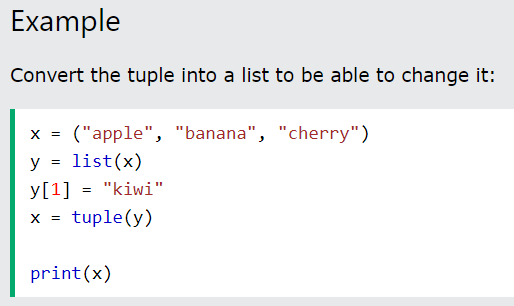
\includegraphics[scale=0.5]{Images/tupleupdate.PNG}
    \caption{Update Tuple}
\end{figure}

Unpacking the tuple \newline
fruits = ("apple", "banana", "cherry") \newline
(green, yellow, red) = fruits


\subsubsection{Set}
\textbf{Properties:}
\begin{itemize}
    \item Unordered, Unordered means that the items in a set do not have a defined order. Set items can appear in a different order every time you use them, and cannot be referred to by index or key.
    \item Unchangeable, Sets are unchangeable, meaning that we cannot change the items after the set has been created.
    \item Duplicates not allowed, Sets cannot have two items with the same value.
\end{itemize}


\textbf{details about some functions}

thisset = \{"apple", "banana", "cherry"\}

\begin{itemize}
    \item Add Items thisset.add("orange")
    \item Add Sets\newline tropical = \{"pineapple", "mango", "papaya"\} thisset.update(tropical)

    \item Add Any Iterable \newline mylist = ["kiwi", "orange"]  thisset.update(mylist)
    \item Remove Item \newline thisset.remove("banana") or thisset.discard("banana")
          \newline \textit{If the item to remove does not exist, remove()/discard() will raise an error}
    \item The clear() method empties the set
    \item The del keyword will delete the set completely example: del listname
\end{itemize}

\textbf{Two approaches of updaing the elements}
一个是建了一个新的set,一个是在原有的set上进行更新
\begin{lstlisting}
set1 = {"a", "b" , "c"}
set2 = {1, 2, 3}

set3 = set1.union(set2)
set1.update(set2)

\end{lstlisting}


\textbf{Set Functions}
\begin{table}
    \begin{tabular}{ll}
        \hline
        \textbf{Method} & \textbf{Description}    \\ \hline
        add()	&Adds an element to the set \\ \hline
        clear()&	Removes all the elements from the set \\ \hline
        copy()	&Returns a copy of the set \\ \hline
        difference()&	Returns a set containing the difference between two or more sets \\ \hline
        difference\_update()&	Removes the items in this set that are also included in another, specified set \\ \hline
        discard()	&Remove the specified item \\ \hline
        intersection()&Returns a set, that is the intersection of two other sets \\ \hline
        intersection\_update()	&Removes the items in this set that are not present in other, specified set(s) \\ \hline
        isdisjoint()&	Returns whether two sets have a intersection or not \\ \hline
        issubset()	&Returns whether another set contains this set or not \\ \hline
        issuperset()	&Returns whether this set contains another set or not \\ \hline
        pop()	&Removes an element from the set \\ \hline
        remove()&	Removes the specified element \\ \hline
        symmetric\_difference()&	Returns a set with the symmetric differences of two sets \\ \hline
        symmetric\_difference\_update()&	inserts the symmetric differences from this set and another \\ \hline
        union()&	Return a set containing the union of sets \\ \hline
        update()	&Update the set with the union of this set and others \\ \hline
    \end{tabular}
\end{table}



\subsubsection{Dictionary}
\begin{itemize}
    \item dictionary.keys() return keys as list

    \item dictionary.values() return values as list
    \item dictionary.update()  thisdict.update({"color": "red"}) The update() method will update the dictionary with the items from a given argument. If the item does not exist, the item will be added.
    \item \textbf{The pop() method removes the item with the specified key name}
    \item \textit{The popitem() method removes the last inserted item (in versions before 3.7, a random item is removed instead)}
    \item \textbf{The del keyword removes the item with the specified key name} \newline del thisdict["model"]

    \item The del keyword can also delete the dictionary completely \newline del thisdict
    \item The clear() method empties the dictionary
    \item Copying dictionary using = will also make a reference as mentioned in tuple. The correct approach to make a copy is using copy() 
\end{itemize}


\subsubsection{collection library}

\subsection{异常处理}

try except else finally \newline
assert,断言。 From W3C School, the assert keyword let you test if a condition in your code return  True, if not, the program will raise an AssertionError.\newline

raise 触发异常

\subsection{OOP}

继承 , 多继承 \newline
函数重写 \newline
类属性  \_\_private\_attrs \newline
类函数:public/private \newline
重载(overload)\newline
重写(overwrite)\newline
覆盖(overrode)\newline

\begin{itemize}
    \item \_\_init\_\_
    \item \_\_new\_\_
\end{itemize}


\subsection{正则表达式}
知识空白,re基础库

\subsection{标准库}
os, sys, re, datetime

\subsection{IO处理}
text, csv, excel, json, 文件写入和读,追加/覆盖...

\section{Django}

补充 Django 基础知识。目前对于Django的一些使用,前后端数据交互,Model,

% \subsection{}

\section{Scrapy}
初步探索Scrapy。

\section{Python 面试}
收集一些Django岗面试题,或者python岗面试题。
[:: - 1]
\end{document}